\documentclass{standalone}
\usepackage{tikz}
\usetikzlibrary{arrows.meta, positioning, quotes, backgrounds}

\begin{document}
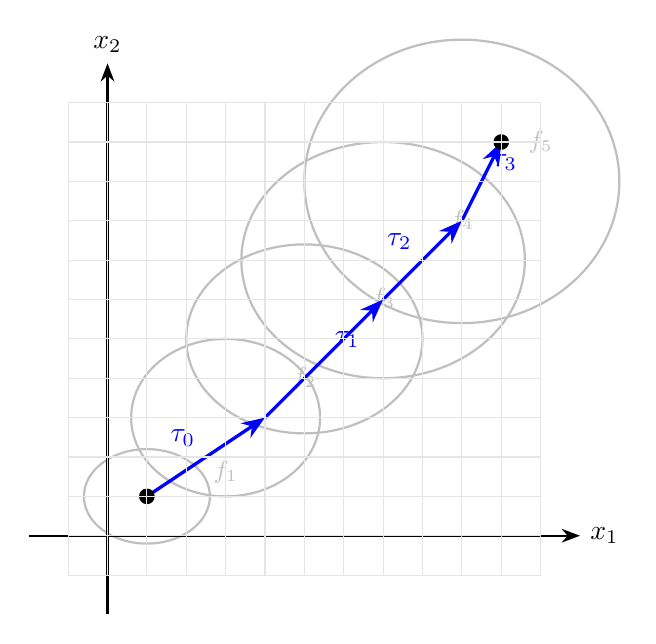
\begin{tikzpicture}[
    >=Stealth,
    axis/.style={thick, ->},
    jump/.style={->, very thick, blue},
    point/.style={circle, fill, inner sep=2pt},
    label/.style={font=\small},
    contour/.style={draw=gray!50, thick}
]

% Draw axes
\draw[axis] (-1, 0) -- (6, 0) node[right] {$x_1$};
\draw[axis] (0, -1) -- (0, 6) node[above] {$x_2$};

% Define points in the trajectory
\coordinate (start) at (0.5, 0.5);
\coordinate (tau0) at (2, 1.5);
\coordinate (tau1) at (3.5, 3);
\coordinate (tau2) at (4.5, 4);
\coordinate (goal) at (5, 5);

% Draw contour plot in the background
\begin{scope}[on background layer]
    % Contour lines (manually defined for simplicity)
    \draw[contour] (0.5, 0.5) ellipse (0.8 and 0.6);
    \draw[contour] (1.5, 1.5) ellipse (1.2 and 1.0);
    \draw[contour] (2.5, 2.5) ellipse (1.5 and 1.2);
    \draw[contour] (3.5, 3.5) ellipse (1.8 and 1.5);
    \draw[contour] (4.5, 4.5) ellipse (2.0 and 1.8);

    % Add labels to contours (optional)
    \node[label, gray!50] at (1.5, 0.8) {$f_1$};
    \node[label, gray!50] at (2.5, 2.0) {$f_2$};
    \node[label, gray!50] at (3.5, 3.0) {$f_3$};
    \node[label, gray!50] at (4.5, 4.0) {$f_4$};
    \node[label, gray!50] at (5.5, 5.0) {$f_5$};
\end{scope}

% Draw trajectory jumps
\draw[jump] (start) to["$\tau_0$" above left] (tau0);
\draw[jump] (tau0) to["$\tau_1$" above right] (tau1);
\draw[jump] (tau1) to["$\tau_2$" above left] (tau2);
\draw[jump] (tau2) to["$\tau_3$" above right] (goal);

% Mark points
\node[point, label={left:Start}] at (start) {};
\node[point, label={above:Goal}] at (goal) {};

% Optional: Add grid for better visualization
\draw[gray!20, step=0.5] (-0.5, -0.5) grid (5.5, 5.5);

\end{tikzpicture}
\end{document}